\documentclass{emulateapj}
%\documentclass[12pt,preprint]{aastex}
\usepackage{graphicx}
\usepackage{float}
\usepackage{amsmath}
\usepackage{epsfig,floatflt}

\usepackage{pgf,tikz}
\usepackage{mathrsfs}
\usetikzlibrary{arrows}

\begin{document}

\title{Diffraction and angular resolution}

\author{Daniel Heinesen}

\email{daniel.heinesen@sf-nett.no}

\altaffiltext{1}{Institute of Theoretical Astrophysics, University of
  Oslo, P.O.\ Box 1029 Blindern, N-0315 Oslo, Norway}


%\date{Received - / Accepted -}

\begin{abstract}
  State problem. Briefly describe method and data. Summarize main results.
\end{abstract}
\keywords{cosmic microwave background --- cosmology: observations --- methods: statistical}

\section{Introduction}
\label{sec:introduction}

Discuss background, physical importance and possibly some history of
the problem that is being studied in this paper.

\section{Theory}
\label{sec:theory}
\subsection{Single Slit}
When the laser hits the single slit the beam interferes with it self and forms a diffraction pattern. The minima of this pattern is given as 

\begin{equation}
\sin \theta_{\min} = \frac{m\lambda}{a}
\end{equation}

Where $m$ is the order of the minimum, $a$ is the width of the slit and $\lambda$ being the wave length of the laser. In this paper the maxima for the single slit was used instead of the minima. So instead of the above expression, an approximation for the maxima had to be used:

\begin{equation}
\sin \theta_{max} \approx \pm (m+1/2)\frac{\lambda}{a}
\end{equation}\label{eq:slitMax}

An unknown wave length can then be calculated as

\begin{equation}
\lambda = \sin \theta_{max}\frac{a}{m+1/2} \approx \theta_{max}\frac{a}{m+1/2}
\end{equation}

\subsection{Paper Clip}
When the single slit is replaced with a single solid object like a paper clip, a diffraction pattern is still observed, but this time inversed. This is due to Babinet's principle, which states: 

If we add a diffraction pattern made by a object \textit{A} and another diffraction pattern made by the complimentary to \textit{A}, the resulting diffraction pattern is as none of the objects existed.

\textbf{Legg til Referanse her!!!}

We can find the angle of the resulting maxima from the following formula

\begin{equation}
\sin \theta_{max} \approx \pm m\frac{\lambda}{a}
\end{equation}\label{eq:paperClipMax}

This can then be used to calculate the width of the paper clip $a$.

\subsection{Diffraction of a Circular Aperture}
Given any type of a circular lens, the lowest image resolution of that lens is determined by Rayleigh criterion

\begin{equation}
\theta_{min} = K\frac{\lambda}{d}
\end{equation}\label{eq:diffLimit}

Where $d$ is the diameter of the lens, $\lambda$ is the wave length of the light and $K$ is some constant. This is the first minimum of the Airy diffraction. For any two objects with a smaller angular distance, there images are indistinguishable from one another, thus appearing as one object.

The constant $K$ need to be found empirically. This is done below.

\subsection{JWST}
The JWST has, as all other optical systems, the resolution limit described above. With the use of the $K$-value we are looking to determine, we can find the angular resolution of JWST with eq. \eqref{eq:diffLimit}. And with the skinny triangle approximation we can find the minimal size of objects JWST can see at different distances:

\begin{equation}
d_{min} = r\theta_{min}
\end{equation}\label{eq:skinny}

\section{Method}
\label{sec:method}


\subsection{Single Slit Experiment}
For the single slit experiment we placed a laser of unknown wavelength, powered by a 4.5 V battery on simple platform and aimed it at a slit with the width of  $a = 100\mu m$. The resulting diffraction pattern was projected on a wall. The distance from the slit to the wall (distance A in fig. \ref{fig:singleSlit}) was measured with a normal household tape measurer.

We then found the distance between the maxima by projecting the diffraction pattern on a piece of white paper and marking every maxima from the 10th on the left to the 10th on the right with a pencil, and then using a ruler to measure the distance between the 10th maximum and the center on each side, and the distance between the 10th maximum on each side, thus getting 3 different measurement which could be used to get a more accurate result.\\

\begin{figure}[H]
\centering
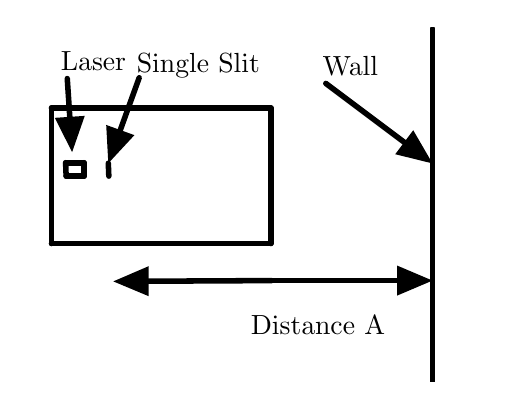
\begin{tikzpicture}[line cap=round,line join=round,>=triangle 45,x=0.7cm,y=0.7cm]
\clip(-3.4514105771947197,-1.1246582774995648) rectangle (4.8753563869437375,5.296334557522694);
\draw [line width=2.pt] (-3.02,3.84)-- (0.96,3.84);
\draw [line width=2.pt] (-3.02,3.84)-- (-3.02,1.38);
\draw [line width=2.pt] (-3.02,1.38)-- (0.96,1.38);
\draw [line width=2.pt] (0.96,3.84)-- (0.96,1.38);
\draw [line width=2.pt] (-2.762868531488555,2.8455024900041326)-- (-2.4269832177375474,2.8455024900041326);
\draw [line width=2.pt] (-2.7535383838843606,2.6029186522950716)-- (-2.4269832177375474,2.6029186522950716);
\draw [line width=2.pt] (-2.4269832177375474,2.8455024900041326)-- (-2.4269832177375474,2.6029186522950716);
\draw [line width=2.pt] (-2.762868531488555,2.8455024900041326)-- (-2.7535383838843606,2.6029186522950716);
\draw [line width=2.pt] (-1.988466280340398,2.836172342399938)-- (-1.9791361327362034,2.6029186522950716);
\draw [line width=2.pt] (3.8931497203992365,5.281674756529493)-- (3.8931497203992365,-1.1246582774995648);
\draw [->,line width=2.pt] (-2.7330803285278455,4.372767094951) -- (-2.6451215225686364,3.0387252045696624);
\draw [->,line width=2.pt] (-1.4283580401329112,4.387426895944201) -- (-1.988466280340398,2.836172342399938);
\draw [->,line width=2.pt] (1.9580559892966374,4.2848082889917904) -- (3.8931497203992365,2.8334879906648416);
\draw [->,line width=2.pt] (0.9758493227521362,0.7078168466506233) -- (-1.8974716719153597,0.6931570456574218);
\draw [->,line width=2.pt] (0.9758493227521362,0.7078168466506233) -- (3.8931497203992365,0.7078168466506236);
\draw (-3.026276348391876,5.047117940638269) node[anchor=north west] {Laser};
\draw (-1.648255055030934,5.017798338651866) node[anchor=north west] {Single Slit};
\draw (1.7234991734054133,4.9591591346790596) node[anchor=north west] {Wall};
\draw (0.4187768850104789,0.2533630158613766) node[anchor=north west] {Distance A};
\end{tikzpicture}
\caption{The experimental set up of the single slit experiment.}
\end{figure}\label{fig:singleSlit}

\subsection{Paper Clip and Anti-Slit}
In this experiment we replaced slit with a paper clip with an unknown width. The rest of the set up was more or less identical as with the single slit experiment, but the laser was moved further back due to the small pattern resulting from the diffraction. This movement of the laser meant that the tape measurer was to short to do the whole measurement. So two the distance from the wall to the paper clip had to be subdivided into a distance from the wall to the edge of the table(Distance C in fig. \ref{fig:setupPaperClip}), and from the edge to the paper clip(Distance B in fig. \ref{fig:setupPaperClip}).

As with the single slit we placed white paper behind the diffraction pattern, and the maxima were marked with a pencil. The distance between the 35th on the left and that on the right of the midpoint was measured with a ruler.

\begin{figure}[H]
\centering
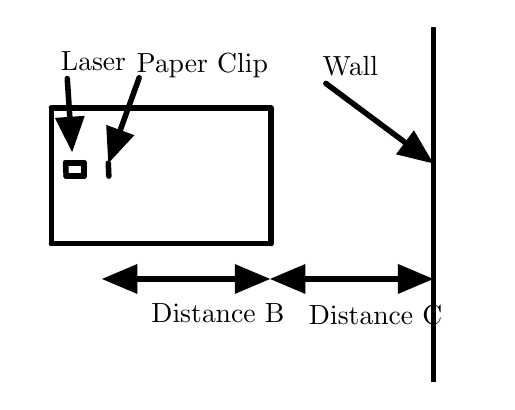
\begin{tikzpicture}[line cap=round,line join=round,>=triangle 45,x=0.7cm,y=0.7cm]
\clip(-3.4514105771947197,-1.1246582774995648) rectangle (4.8753563869437375,5.296334557522694);
\draw [line width=2.pt] (-3.02,3.84)-- (0.96,3.84);
\draw [line width=2.pt] (-3.02,3.84)-- (-3.02,1.38);
\draw [line width=2.pt] (-3.02,1.38)-- (0.96,1.38);
\draw [line width=2.pt] (0.96,3.84)-- (0.96,1.38);
\draw [line width=2.pt] (-2.762868531488555,2.8455024900041326)-- (-2.4269832177375474,2.8455024900041326);
\draw [line width=2.pt] (-2.7535383838843606,2.6029186522950716)-- (-2.4269832177375474,2.6029186522950716);
\draw [line width=2.pt] (-2.4269832177375474,2.8455024900041326)-- (-2.4269832177375474,2.6029186522950716);
\draw [line width=2.pt] (-2.762868531488555,2.8455024900041326)-- (-2.7535383838843606,2.6029186522950716);
\draw [line width=2.pt] (-1.988466280340398,2.836172342399938)-- (-1.9791361327362034,2.6029186522950716);
\draw [line width=2.pt] (3.907809521392438,5.281674756529493)-- (3.907809521392438,-1.1246582774995648);
\draw [->,line width=2.pt] (-2.7330803285278455,4.372767094951) -- (-2.6451215225686364,3.0387252045696624);
\draw [->,line width=2.pt] (-1.4283580401329112,4.387426895944201) -- (-1.988466280340398,2.836172342399938);
\draw [->,line width=2.pt] (1.9580559892966374,4.2848082889917904) -- (3.907809521392438,2.8334879906648416);
\draw [->,line width=2.pt] (-0.7833267964320458,0.7371364486370263) -- (-2.102708885820181,0.7371364486370263);
\draw (-3.026276348391876,5.047117940638269) node[anchor=north west] {Laser};
\draw (-1.648255055030934,5.017798338651866) node[anchor=north west] {Paper Clip};
\draw (1.7234991734054133,4.9591591346790596) node[anchor=north west] {Wall};
\draw (-1.384378637153307,0.4732600307593992) node[anchor=north west] {Distance B};
\draw [->,line width=2.pt] (-0.7833267964320458,0.7371364486370263) -- (0.9465297207657333,0.7371364486370262);
\draw [->,line width=2.pt] (2.4271696210790856,0.7371364486370262) -- (0.9465297207657333,0.7371364486370262);
\draw [->,line width=2.pt] (2.4271696210790856,0.7371364486370262) -- (3.907809521392438,0.7371364486370262);
\draw (1.4742825565209876,0.4292806277797947) node[anchor=north west] {Distance C};
\end{tikzpicture}
\caption{The experimental set up in the paper clip experiment.}
\end{figure}\label{fig:setupPaperClip}

\subsection{Diffraction by a Circular Aperture}
For this experiment we shinned laser of known wave length into an optic fibre. The fibre was connected to a collimator tube with dampening filter -- so to not destroy the camera. The tube was meant to ensure that the beam exiting on the end was as parallel as possible. To then focus the beam, we placed a double lens after the tube. We then placed a microscope objective in front of a lens, which magnified the light 20x. Lastly a monochromatic camera connected to a computer was placed in front of the objective to capture the diffraction pattern.

We then carefully measured the diameter of the lens with a ruler.

The objective had to be placed in the focal point of the lens, $f = 100$ mm. To ensure that the beam was focused and was hitting the objective, we placed a piece of white paper in front of the objective. We then adjusted the lens until the beam hit the objective. The paper was then moved back and forward to see if the light was most concentrated at the focal point. 

Having a picture of the Airy pattern, we could count the number of pixels from the center of the disc to the first minimum, as seen in figure \ref{fig:airy}. Knowing the size of each pixel and the distance from the objective and the camera, we could calculate the angle of the first minimum. From the angle of the first minimum, a value for $K$ was calculated.

\begin{figure}
\centering
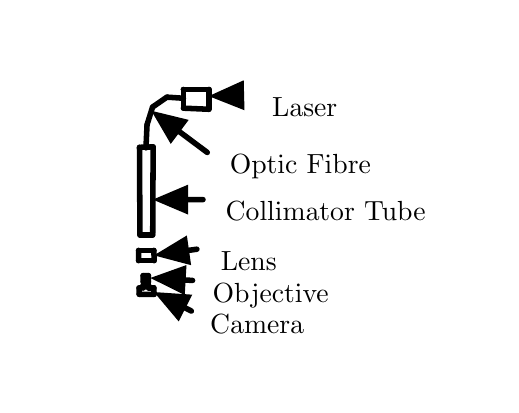
\begin{tikzpicture}[line cap=round,line join=round,>=triangle 45,x=0.7cm,y=0.7cm]
\clip(-1.1857969150189058,0.564677444748752) rectangle (7.212033122512422,7.040468917352141);
\draw [line width=2.pt] (2.1,5.92)-- (1.64,5.92);
\draw [line width=2.pt] (2.1,5.92)-- (1.64,5.92);
\draw [line width=2.pt] (1.64,5.92)-- (1.64,5.58);
\draw [line width=2.pt] (1.64,5.58)-- (2.1,5.56);
\draw [line width=2.pt] (2.1,5.92)-- (2.1,5.56);
\draw [line width=2.pt] (1.64,5.76)-- (1.34,5.78);
\draw [line width=2.pt] (1.34,5.78)-- (1.08,5.6);
\draw [line width=2.pt] (1.08,5.6)-- (0.98,5.28);
\draw [line width=2.pt] (0.98,5.28)-- (0.96,4.86);
\draw [line width=2.pt] (1.0904707609684874,4.877174417231538)-- (0.8431895330994198,4.869681046690051);
\draw [line width=2.pt] (0.8431895330994198,4.869681046690051)-- (0.8506829036409067,3.2810864918948313);
\draw [line width=2.pt] (1.0904707609684874,4.877174417231538)-- (1.0829773904270004,3.2810864918948313);
\draw [line width=2.pt] (0.8506829036409067,3.2810864918948313)-- (1.0829773904270004,3.2810864918948313);
\draw [line width=2.pt] (0.8266285825814105,3.000220845407801)-- (1.1041712979437268,3.000220845407801);
\draw [line width=2.pt] (0.8266285825814105,3.000220845407801)-- (0.8262947059116466,2.812922522802634);
\draw [line width=2.pt] (0.8262947059116466,2.812922522802634)-- (1.1088659806223602,2.812922522802634);
\draw [line width=2.pt] (1.1088659806223602,2.812922522802634)-- (1.1041712979437268,3.000220845407801);
\draw [line width=2.pt] (0.9087113277022714,2.5421250512048674)-- (1.004546842556573,2.541129751750464);
\draw [line width=2.pt] (0.9087113277022714,2.5421250512048674)-- (0.9103167128615315,2.4270617000143613);
\draw [line width=2.pt] (0.9103167128615315,2.4270617000143613)-- (1.0056047261328107,2.4269784146127376);
\draw [line width=2.pt] (1.0056047261328107,2.4269784146127376)-- (1.004546842556573,2.541129751750464);
\draw [line width=2.pt] (0.9096320114748135,2.369913557248523)-- (1.0081985832857296,2.369913557248523);
\draw [line width=2.pt] (1.0081985832857296,2.369913557248523)-- (1.0081985832857296,2.320630271343065);
\draw [line width=2.pt] (1.0081985832857296,2.320630271343065)-- (1.1041712979437268,2.320630271343065);
\draw [line width=2.pt] (1.1041712979437268,2.320630271343065)-- (1.1067651550966455,2.2013128423087984);
\draw [line width=2.pt] (1.1067651550966455,2.2013128423087984)-- (0.8370040111930859,2.203906699461717);
\draw [line width=2.pt] (0.8370040111930859,2.203906699461717)-- (0.834410154040167,2.318036414190146);
\draw [line width=2.pt] (0.834410154040167,2.318036414190146)-- (0.9122258686277324,2.320630271343065);
\draw [line width=2.pt] (0.9122258686277324,2.320630271343065)-- (0.9096320114748135,2.369913557248523);
\draw [->,line width=2.pt] (1.784126456141933,1.8994295337607234) -- (1.1058422520405622,2.2437663828886953);
\draw [->,line width=2.pt] (1.8063427026301484,2.4548356959661053) -- (1.0398821987867215,2.499268188942536);
\draw [->,line width=2.pt] (1.8840995653389019,3.021349981415595) -- (1.1064399862523078,2.90970961306294);
\draw [->,line width=2.pt] (1.9951807977799783,3.9211079641883138) -- (1.0859823941524378,3.921152285412984);
\draw [->,line width=2.pt] (2.0729376604887317,4.776433453984602) -- (1.0589869320234415,5.532758182475013);
\draw [->,line width=2.pt] (2.5505869599853597,5.809488915686613) -- (2.1,5.798380792442505);
\draw (3.0722577518983876,5.946385426547002) node[anchor=north west] {Laser};
\draw (2.3034423259272097,4.9262264959314) node[anchor=north west] {Optic Fibre};
\draw (2.2295177657376732,4.068701597732778) node[anchor=north west] {Collimator Tube};
\draw (2.1408082935102293,3.152037051382526) node[anchor=north west] {Lens};
\draw (1.992959173131157,2.575425481904142) node[anchor=north west] {Objective};
\draw (1.948604437017435,2.0135988244636653) node[anchor=north west] {Camera};
\end{tikzpicture}
\caption{The experimental set up for the diffraction of a circular aperture experiment.}
\end{figure}\label{fig:setupAiry}

\subsection{Arago spot}
The lens, objective and camera was then removed and replaced by a small circular piece of plastic. The resulting pattern was projected on to the wall.

\subsection{JWST} 
Having found the diffraction limit of a lens, we were able to find the limit for the James Webb Space Telescope(JWST) from \eqref{eq:diffLimit}. 

\subsection{Uncertainties}
\subsubsection{Single slit}
The distance between the slit and the wall was measured with a tape measurer. Due to the flexible nature of the tape measurer, the distance was not measured in a straight line, giving rise to a small uncertainty. A uncertainty of $\pm 0.5 cm$ was added to the distance.

It was also difficult to ensure that the measurement was done in a horizontal line, normal to the wall. The set up it self also contributed to the uncertainty of the measurements: to get a consistent distance between the maxima the laser had to be normal to the wall, and the slit in the center of the laser beam. \\

Our measurement of the distance of the extrema of the diffraction pattern was done quite crude, so both the marking of the maxima on the paper and the measuring with the ruler lead to uncertainty. We took extension of the maxima to be half that of the distance between two adjacent maxima. The error in measurement was estimated to at most one quarter that of this distance, giving us quite a large uncertainty. The error of the ruler was determined to insignificant compared to that of the marking, so only that uncertainty was kept.

To compensate for all these uncertainties, an uncertainty of $\pm 0.1 cm$ was added to the distance to the 10th maxima.


\subsubsection{Paper clip}
Our first measurement was from the wall to the table used for the laser and paper clip. Here the same problem as the measurement for the single slit appears, as the tape measurer bends under its own weight, thus measuring a slightly longer distance. 

Our second measurement was from the end of the table to the paper clip. Here we placed the tape measurer on the table surface, thus there was no bend in the measurer, giving a more precise measurement. 

Since two measurements were done, an uncertainty arose from the difficulty in starting the second measurement where the first ended. So a small uncertainty was added to the second measurement to compensate for this.

Due to the short distance from the paper clip to the wall, the maxima of the diffraction pattern were close together, making the marking of the maxima quite uncertain. This together with uncertainty in the ruler, did that we added certainty of $\pm 0.2 cm$. 

\subsubsection{Diffraction of a Circular Aperture}
Three measurements was the main sources for uncertainty in this experiment.

We measured the distance between the lens and objective with a ruler. This measurement was taken from the start of the objective to the center of the lens. The uncertainty was estimated to be some $\pm 0.5 cm$.

The width of the lens was also measured with a ruler, but was easier to measure, giving only an uncertainty of $\pm 0.2$.

The Airy Disc was contained in very few pixels in the picture. The point of the first minimum may be in-between two pixels, giving an uncertainty of a whole pixel. The center of the Airy disc may also not be in one single pixel, but since the area of the disc is much larger than the point of the minimum, this does not contribute so much to the total uncertainty.

\section{Results}
\label{sec:results}

\subsection{Measurements}
\subsubsection{Single slit}

\begin{table}[H]
\begin{tabular}{ c c c }
Measurement done & Measured value & Unit\\
\hline
Distance laser to wall & $183 \pm 0.5$ & cm \\
Distance from midpoint to 10th max & $12.25 \pm 0.1$ & cm\\
Distance from 10th max to midpoint & $12.40 \pm 0.1$ & cm\\
Distance from 10th max to 10th max & $24.70 \pm 0.1$ & cm\\
Average distance to 10th max & $12.33 \pm 0.23$ & cm\\
Calculated wave length of laser\eqref{eq:waveLenghtLaser} & $641 \pm 12.29$ &nm 
\end{tabular}
\caption{The measurements for the single slit experiment.}
\end{table}\label{tab:dataSingleSlit}

\subsubsection{Paper clip}

\begin{table}[H]
\begin{tabular}{ c c c }
Measurement done & Measured value & Unit\\
\hline
Distance from paper clip to end of table & $102.0 \pm 0.5$ & cm \\
Distance from end of table to wall & $120.5 \pm 0.5$ & cm \\
Distance from 35th max to 35th max & $11.6 \pm 0.2$ & cm\\
Calculated width of Paper Clip\eqref{eq:widthPaperClip} & $0.4743 \pm 0.01281$ & mm
\end{tabular}
\caption{The measurements for the paper clip experiments.}
\end{table}\label{tab:dataPaperClip}

\subsubsection{Diffraction of a Circular Aperture}

\begin{table}[H]
\begin{tabular}{ c c c }
Measurement done & Measured value & Unit\\
\hline
Wave length of laser & $635$ & nm \\
Distance from lens to objective & $10 \pm 0.5$ & cm\\
Width of lens & $5.0 \pm 0.2$ & cm\\
Pixels from center to first minimum & $3 \pm 1$ & px\\
Size of pixels & $6$ & $\mu$m/px\\
Magnification & 20x & -\\
Distance from center to first minimum & $\frac{18 \pm 6}{20}$& $\mu$m\\
Calculated value for $K$\eqref{eq:K} &  $0.71 \pm 0.238$ & -
\end{tabular}
\caption{The measurements for the circular diffraction.}
\end{table}\label{tab:dataAiry}

\begin{figure}[H]
\centering
\includegraphics[scale=0.4]{Airy3zoomed2.png}
\caption{Zoomed in picture of the Airy disc. The distance from the center of the disc to the first minimum is marked in red. The distance is 3 pixels.}
\end{figure}\label{fig:airy}

\subsubsection{JWST}
\begin{table}[H]
\centering
\begin{tabular}{ c c c }
Mirror Size & Frequencies \\
\hline
6 m & 600 nm - 28.5 $\mu$m 
\end{tabular}
\caption{Data for the James Webb Space Telescope}
\end{table}\label{tab:dataJWST}

\begin{table}[H]
\centering
\begin{tabular}{ c c c }
Target & Distance $r$ & Smallest Size $r_{min}$ \\
\hline
Near-Earth orbit to Earth & 540 km &$8.1 \pm 2.7$ cm \\
Earth to sun & 1 AU & $22.44 \pm 7.5$ km \\
Solar System to Galactic Center & 8.5 pc & $3.9\cdot 10^7 \pm 1.3\cdot 10^7$ km \\
Milky Way to galaxy formation &  4 billion ly & $184 \pm 61.5$ pc 
\end{tabular}
\caption{The smallest size the JWST can see at different distances. A Skinny triangle approximation is used with the angular resolution found in \eqref{JWSTDiffLimit}.}
\end{table}\label{tab:visionJWST}


\subsection{Calculation}
\subsubsection{Single slit}


From the data in \ref{tab:dataSingleSlit} the angle can be estimated as

\begin{equation}
\theta_{max} \approx \arctan\left( \frac{12.33}{183} \pm 0.0013 \right) = 0.0673 \pm 0.00129
\end{equation}

Which gives 

\begin{equation}
\lambda \approx (0.0673 \pm 0.00129) \cdot \frac{100}{10 +1/2}\text{ }\mu \text{m} 
\end{equation}
\begin{equation}
= 0.641\pm 0.01229\text{ }\mu \text{m} = 641 \pm 12.29 \text{ nm}
\end{equation}\label{eq:waveLenghtLaser}

So based on this experiment, the laser should have a wave length of $641 \pm 12.29 \text{ nm}$.

\subsubsection{Paper Clip}

The width of the paper clip can be found with the use of \eqref{eq:paperClipMax}. The width is given as

\begin{equation}
a \approx \frac{m \lambda}{\theta_{max}}
\end{equation}

We found the angle as

\begin{equation}
\theta_{max} \approx \arctan\left(\frac{5.8}{122.5} \pm 0.00086\right) =0.0473 \pm 0.0009
\end{equation}

Giving a a estimated width of

\begin{equation}
a \approx \frac{35\cdot (641 \pm 12.29)}{0.0473 \pm 0.0009} \text{ nm}
\end{equation} 

\begin{equation}
= 0.4743 \pm 0.01281 \text{ mm}
\end{equation}\label{eq:widthPaperClip}

Which gives us a width of the paper clip of $0.4743 \pm 0.01281 \text{ mm}$.

\subsubsection{Diffraction of a Circular Aperture}

With the use of \eqref{eq:diffLimit} a value for $K$ was calculated.

\begin{equation}
K = \frac{\theta_{min} d}{\lambda}
\end{equation}

The angle was found as

\begin{equation}
\theta_{min} = \arctan\left(\frac{18/20}{100000} \pm 3.005\cdot 10^{-6} \right)
\end{equation}
\begin{equation}
= 9\cdot 10^{-6} \pm 3.005\cdot 10^{-6}
\end{equation}

We then used this to calculate $K$

\begin{equation}
K = \frac{9\cdot 10^{-6} \pm 3.005\cdot 10^{-6}}{635}\cdot(5\cdot10^7 \pm 2\cdot10^6)
\end{equation}
\begin{equation}
= 0.71 \pm 0.238
\end{equation}\label{eq:K}

So the estimated value was $K = 0.71 \pm 0.238$

\subsubsection{JWST}
From the above results, mainly \eqref{eq:K} we can find the diffraction limit of the James Webb Space Telescope:

\begin{equation}
\theta_{min} = (1.417 \pm 0.474) \cdot \frac{635 \text{ nm}}{6 \text{ m}}
\end{equation}
\begin{equation}
= 1.5\cdot 10^{-7} \pm 5.016\cdot 10^{-8}
\end{equation}\label{JWSTDiffLimit}

This can then be used to find the smallest physical sizes the JWST can see at different distances, with the use of the skinny triangle approximation \eqref{eq:skinny}. These distances can be found in table \eqref{tab:visionJWST}
\section{Conclusions}
\label{sec:conclusions}

Summarize results. Discuss their importance, referring to the
discovery to the initial seeds for structure formation. Mention that
these results are in good agreement with expectations from
inflationary theory.



%\begin{figure}[t]
%
%\mbox{\epsfig{figure=filename.eps,width=\linewidth,clip=}}
%
%\caption{Description of figure -- explain all elements, but do not
%draw conclusions here.}
%\label{fig:figure_label}
%\end{figure}


%
%\begin{deluxetable}{lccc}
%%\tablewidth{0pt}
%\tablecaption{\label{tab:results}}
%\tablecomments{Summary of main results.}
%\tablecolumns{4}
%\tablehead{Column 1  & Column 2 & Column 3 & Column 4}
%\startdata
%Item 1 & Item 2 & Item 3 & Item 4
%\enddata
%\end{deluxetable}



\begin{acknowledgements}
  Who do you want to thank for helping out with this project?
\end{acknowledgements}

\begin{thebibliography}{}

\bibitem[G{\'o}rski et al.(1994)]{gorski:1994} G{\'o}rski, K. M.,
  Hinshaw, G., Banday, A. J., Bennett, C. L., Wright, E. L., Kogut,
  A., Smoot, G. F., and Lubin, P.\ 1994, ApJL, 430, 89

\end{thebibliography}


\end{document}